\section{Обсуждение результатов}
\subsection{Изучение Si}
Измерение проводилось в нескольких переустановках образца и разных расстояниях $D$ и углах $2\theta_D$.
Также для оценки возможности использования рефлексов отстоящих от центра детектора съемка фриделевской пары $\hkl(-9 7 1)/\hkl(9 -7 -1)$ была проведена при положении детектора $2\theta_D = \pm 97.5\degree$, что является крайним положением для $D = 128.5\unit{мм}$, которое отличается от идеального почти на $0.8\degree$.
Исследование фриделевской пары $\hkl(3 -3 1)/\hkl(-3 3 -11)$ показало разницу координат $Y$ всего 4~пикс.
Среднее значение отклонение экспериментально полученных значений $2\theta$ от эталонных составило $0.0003\degree$, а среднее значение ПЭЯ отличается от эталонного на $0.0001\unit{\AA}$.
Относительная погрешность определения $d$ и ПЭЯ составила $5 \times 10^{-5}$.
\subsection{Изучение Ge}
На монокристалле Ge проводили контроль воспроизводимости установки образца и детектора.
Для этого было выполнено несколько переустановок образца, в том числе с коррекцией ориентации кристалла, изменением $D$ и угла $2\theta_D$.
При $D = 138.6\unit{мм}$ изучены рефлексы $\hkl(5 -11 -1)$ и $\hkl(1 -11 -5)$ с существенно отличными углами выведения в отражающее положение $(\varphi, \omega)$.
Для оценки возможности использования рефлексов, значительно отстоящих от центра детектора, съемка рефлекса $\hkl(7 -7 -7)$ была проведена при двух разных значениях $2\theta_D$.
Причем положение $\pm 99.9\degree$ отличалось от идеального почти на $1\degree$.
Исследование фриделевской пары $\hkl(3 -3 11)/\hkl(-3 3 -11)$ показало хороший уровень точности выведения рефлексов на экваториальную плоскость: разница координат $Y$ не превысила $\approx 7\unit{пикс.}$, что составляет $\approx 0.4\degree$.
В результате обработки профилей рефлексов были получены координаты максимумов и по формуле~\ref{eq:bond2} определены углы $2\theta$, а из них рассчитаны значения $d$ и ПЭЯ.
Среднее отклонение полученных значений $2\theta$ от теоретических составило $0.004\degree$, что соответствует точности гониометра.
Если ориентироваться на полученную величину, то относительная погрешность определения межплоскостного расстояния $\Delta d / d = 6 \times 10^{-5}$.
Таким образом, абсолютную погрешность определения ПЭЯ для Ge можно оценить как $0.0003\unit{\AA}$.
Среднее значение $a_\text{Ge} = 5.6579\unit{\AA}$ отличается от эталонного значения меньше, всего на $0.0001\unit{\AA}$.
\subsection{Изучение \YEu}
При выборе рефлекса, подходящего для уточнения ПЭЯ, мы столкнулись с проблемой оценки его интенсивности из-за хиральности точечной группы симметрии кристалла.
Так, например, теоретические значения структурной амплитуды рефлексов $\hkl(6 8 20)$ и $\hkl(8 6 20)$ соотносятся как 7 к 1.
Естественно, предпочтительно использовать наиболее интенсивное отражение.
Для решение этой проблемы предварительная съемка кристалла была скорректирована --- расстояние $D$ уменьшено до $60\unit{мм}$, а углы $2\theta_D$ увеличены до $\pm 75\degree$.
В результате были построены сечения обратного пространства, захватывающие область углов $2\theta = \range{95\degree}{100\degree}$.
Сопоставление интенсивностей рефлексов с результатами вычислений программы позволило выбрать оптимальные индексы.
По такой схеме было проведено исследование 5 монокристаллов.
Значения ПЭЯ лежат в интервале $\range{10.6902}{10.7045}\unit{\AA}$.
Разница крайних значений составляет $0.0143\unit{\AA}$.
Это значительно превосходит абсолютную погрешность определения ПЭЯ, равную $0.0007\unit{\AA}$.
Таким образом, можно однозначно утверждать, что синтезированный продукт не однороден.

Для оценки соотношения Y/Eu в изученных монокристаллах \YEu~можно использовать правило Вегарда.
Для построения соответствующей прямой были использованы литературные данные~\cite{Swanson:1954,Morris:1984}.

Для проведения РСтА расчет стратегии съемки для накопления полного массива данных производился для каждого кристалла автоматически с учетом его симметрии $(m\overline{3})$ по предварительно определенной матрице ориентации с использованием пакета программ APEX3.
Далее проводили интегрирование экспериментальных интенсивностей и вводили поправки на поглощение.
Структуры решены с помощью программы SHELXT~\cite{Sheldrick:2015:shelxt} и уточнены с SHELXL~\cite{Sheldrick:2015:shelxl} в графическом интерфейсе OLEX2~\cite{Dolomanov:2009}.
Параметры атомных смещений были уточнены в анизотропном приближении.

В результате установлено, что все изученные кристаллы изоструктурны и представляют собой твердые растворы \YEu, причем смешанными оказываются обе позиции металла.
\begin{figure}[ht!]
    \centering
    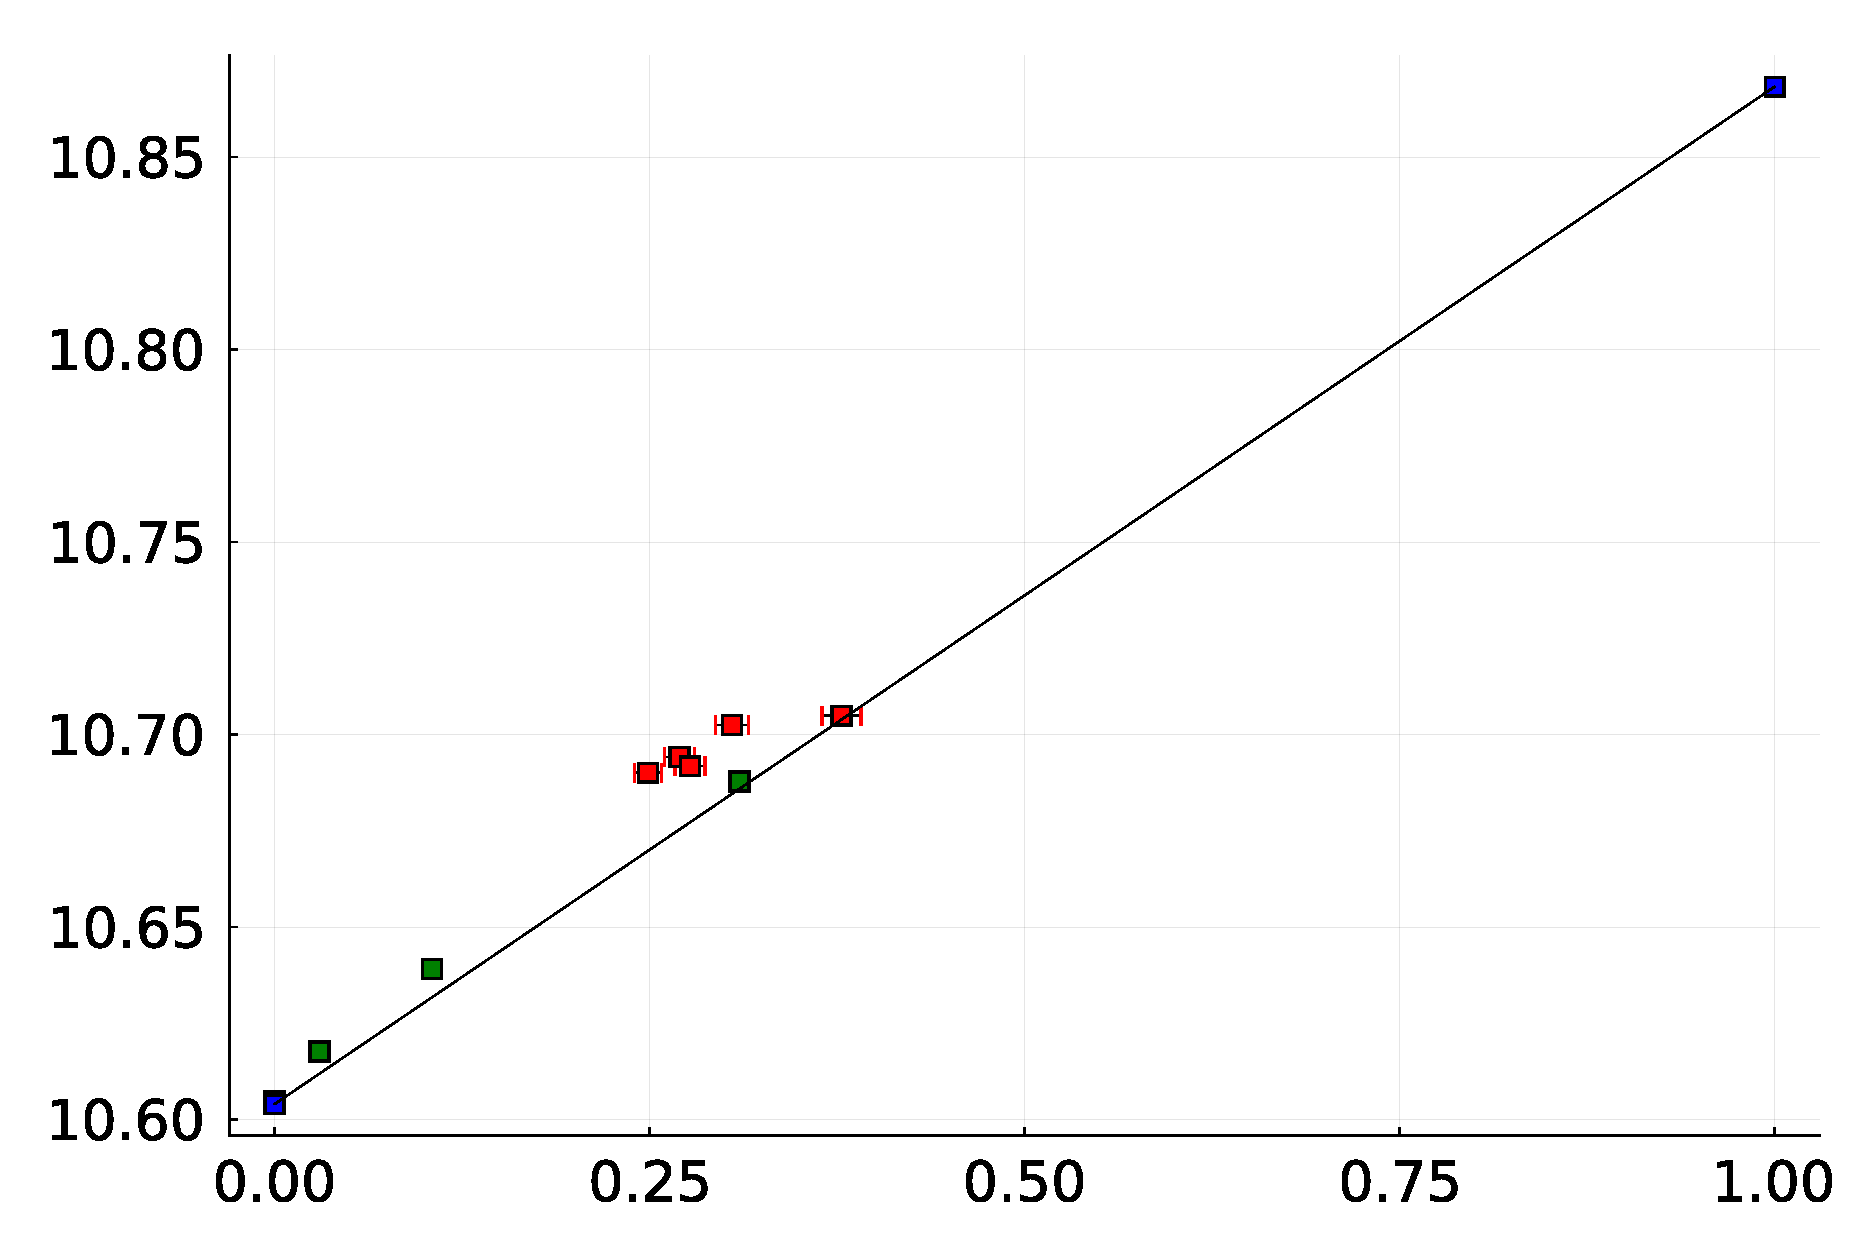
\includegraphics[width=0.8\textwidth]{YEu.pdf}
    \caption{Зависимость ПЭЯ \YEu~от мольной доли $x$.}
    \label{fig:YEu}
\end{figure}

\subsection{Оценка и учет эксцентриситета образца Si}
Несмотря на тщательную центрировку образца, в том числе с контрольными разворотами по оси $\omega$, крайне сложно точно определить его центр, особенно при неопределенной форме кристалла.
Можно ожидать, что при повороте вокруг оси $\omega$ центр образца движется по окружности, а сам образец описывает торообразную поверхность.
Подобную картину можно ожидать и при повороте образца вокруг оси $\varphi$.
Так как для использованного гониометра паспортное значение диаметра сферы сведения осей составляет $7\unit{мкм}$, центр образца при повороте вокруг обеих осей движется по достаточно сложной траектории.

Для оценки смещений центра образца при повороте вокруг оси $\varphi$, среди доступных для измерения рефлексов типов $\hkl{11 3 1}$, $\hkl{9 7 1}$ и $\hkl{9 5 5}$, было выбрано 10 вариантов, у которых значения $\omega$ лежат в интервале $\range{-82\degree}{95\degree}$.
Это примерно соответствует позиции образца при центрировании.
Все съемки проведены при одном положении детектора: $2\theta_D = -96.7\degree$, $D = 128.53\unit{мм}$.

Для оценки эксцентриситета при повороте вокруг оси $\omega$, были отобраны случаи, когда значения $\varphi$ лежат в интервале $\range{283.6\degree}{300.7\degree}$.
При этом соответствующие им углы $\omega$ лежат в интервале $\range{63.3\degree}{296.5\degree}$.
Область $\pm 60\degree$ недоступна из-за геометрических ограничений гониометра.
Графики зависимости координат от углов поворота представлены на графике~\ref{fig:eccentrSi}.

\begin{figure}[ht!]
    \centering
    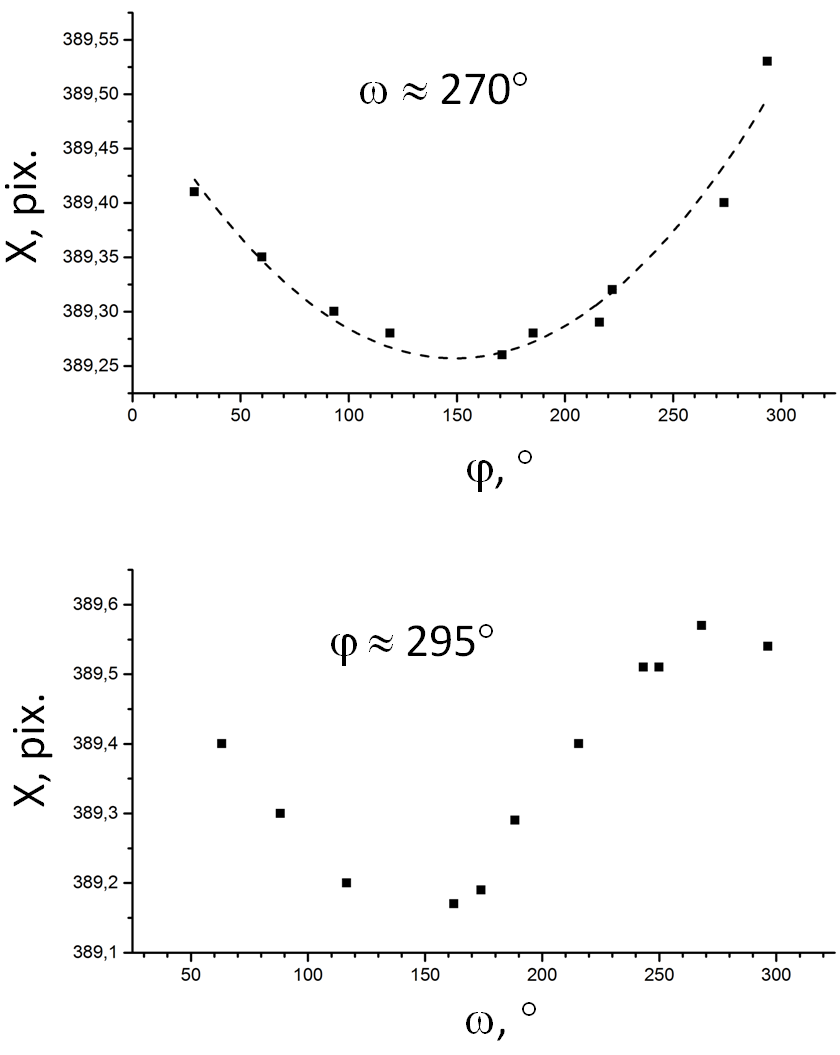
\includegraphics[width=0.8\textwidth]{eccentrSi.png}
    \caption{Смещение максимумов дифракционных отражений $\hkl(11 3 1)$, $\hkl(9 7 1)$ и $\hkl(9 5 5)$ по оси $X$ детектора из-за эксцентриситета образца: $a$ --– зависимость координаты $X$ от угла $\varphi$ (значения углов $\omega \approx 270\degree$); $b$ --- зависимость координаты $X$ от угла $\omega$ (значения углов $\varphi$ лежат в интервале от $\range{283.6\degree}{300.7\degree}$).}
    \label{fig:eccentrSi}
\end{figure}

Таким образом, проведенные два эксперимента показали одинаковую картину для эксцентриситетов, связанных с поворотами образца вокруг осей $\varphi$ и $\omega$.
При измерении ПЭЯ наиболее разумно исключить влияние именно последнего, тогда далее можно использовать подход, описанный выше~\cite{Ponomarev:1969}.

Среди всех вариантов рефлексов были выделены 5 фриделевских пар.
\subsection{Учет эксцентриситета для Si}
При произвольном выборе рефлексов расчет по~\ref{eq:bond2} приводит к значениям угла $2\theta$ в интервале $\range{96.722\degree}{96.747\degree}$.
Учет эксцентриситета по формуле~\ref{eq:bond4} уменьшает интервал значений до $\range{96.730\degree}{96.736\degree}$, а отклонения от теоретического значения не превышают $0.004\degree$.
Использование рефлексов с близкими значениями $\varphi = 66.31\degree, \, 59.35\degree$ позволяет пренебречь эксцентриситетом, связанным с поворотам вокруг оси $\varphi$.
Конечные результаты уточнения представлены в таблице~\ref{tab:Si:eccentr}.
\begin{table}[ht!]
    \centering
    \begin{tabular}{ |c|c| }
        \hline
        $2\theta$ & $96.732\degree$ \\
        $d$ & $0.47452 (3)\unit{\AA}$ \\
        $\Delta d / d$ & $6.2 \times 10^{-5}$ \\
        $a$ & $5.4311 (3)\unit{\AA}$ \\
        \hline
    \end{tabular}
    \caption{Результаты измерений ПЭЯ Si с учетом эксцентриситета.}
    \label{tab:Si:eccentr}
\end{table}

Можно отметить, что полученное значение ПЭЯ отклоняется от эталонного на $0.00006\unit{\AA}$.
Т. е. относительная разница составляет $1\times 10^{-5}$.
Еще раз подчеркнем, что результат получен лишь при частичном учете эксцентриситета, связанного с поворотом кристалла вокруг оси $\varphi$.
Чтобы полностью исключить такое влияние можно вывести одно из кристаллографических направлений вдоль оси $\omega$.
Тогда измерения можно проводить на рефлексах типа $hk0$.
При использовании трехкружного гониометра для образца такая проблема не возникает.
В нашем случае угол $\chi$ --- фиксирован, а штатные гониометрические головки предполагают только линейные смещения образца.
\subsection{Учет эксцентриситета для Ge}
Для устранения эксцентриситета, связанного с поворотом кристалла вокруг оси $\varphi$, монокристалл Ge был смонтирован на оригинальной гониометрической головке, имеющей возможность поворота образца вокруг одной оси на $\pm 10\degree$ (далее гониометрическая $\chi$--головка).
После определения ориентации кристалла были рассчитаны углы для выведения кристаллографического направления вдоль оси $\omega$. Алгоритм этого процесса описан в~\cite{Kudryavtsev:2024:eccentr}.

Расчеты для монокристалла Ge показали, что вдоль оси $\omega$ можно вывести направление $b$, так как для него значения угла $\chi = 2.2\degree$.
После поворота, исследование по нашей методике было проведено по рефлексам типа $\hkl{10 0 6}$.
Им соответствовало значение угла $2\theta = 93.943\degree$.
Все рефлексы регистрировались при одинаковых значениях угла $\varphi = -179.06\degree$.
Геометрические ограничения позволили отснять при $2\theta_D = \pm 93.9\degree$ только 12 из 16 теоретически возможных рефлексов.
При произвольных сочетаниях рефлексов значения $2\theta$, вычисленные по~\ref{eq:bond2} лежат в интервале $\range{93.935\degree}{93.958\degree}$.
Максимальные отклонения от теоретического значения достигают $0.015\degree$.
При использовании формулы~\ref{eq:bond4} углы $2\theta$ укладываются в интервал $\range{93.943\degree}{93.945\degree}$.
Отклонения от теоретического значения в таком случае не превышают $0.001\degree$.
Финальные значения для Ge представлены в таблице~\ref{tab:Ge:eccentr}.
Отклонение полученного значения ПЭЯ от теоретического составляет $0.0001\unit{\AA}$.
\begin{table}[ht!]
    \centering
    \begin{tabular}{ |c|c| }
        \hline
        $2\theta$ & $93.945\degree$ \\
        $d$ & $0.48515 (3)\unit{\AA}$ \\
        $\Delta d / d$ & $6.5 \times 10^{-5}$ \\
        $a$ & $5.6578 (4)\unit{\AA}$ \\
        \hline
    \end{tabular}
    \caption{Результаты измерений ПЭЯ Ge с учетом эксцентриситета.}
    \label{tab:Ge:eccentr}
\end{table}

Анализ координат $Y$ рефлексов Ge позволяет оценить точность выведения направления $b$ вдоль оси $\omega$.
Для этого можно построить зависимости $Y(\omega)$ для экспериментов, проведенных при дух симметричных положениях детектора $2\theta_D = \pm 93.9\degree$.
Она представлена на графике~\ref{fig:eccentrGe}.
В обоих случаях зависимости хорошо описываются синусоидами, но при $2\theta_D = -93.9\degree$ фаза сдвигается на $\theta$, а при $2\theta_D = +93.9\degree$ на $\theta + 180\degree$.
Для обработки всех рефлексов одновременно значения сдвигов вычитались из первичных значений $\omega$.
Из построенной аппроксимации следует, что максимальное отклонение направления $b$ от оси $\omega$ составляет $\approx 2.2\unit{пикс.}$, что эквивалентно $0.13\degree$.
Такое значение соответствует цене нониуса дуги гониометрической головки.
Так как отклонение лежит в ее плоскости, то можно утверждать что оно связано преимущественно с погрешностью установки угла $\chi$, а не $\varphi$.

\begin{figure}[ht!]
    \centering
    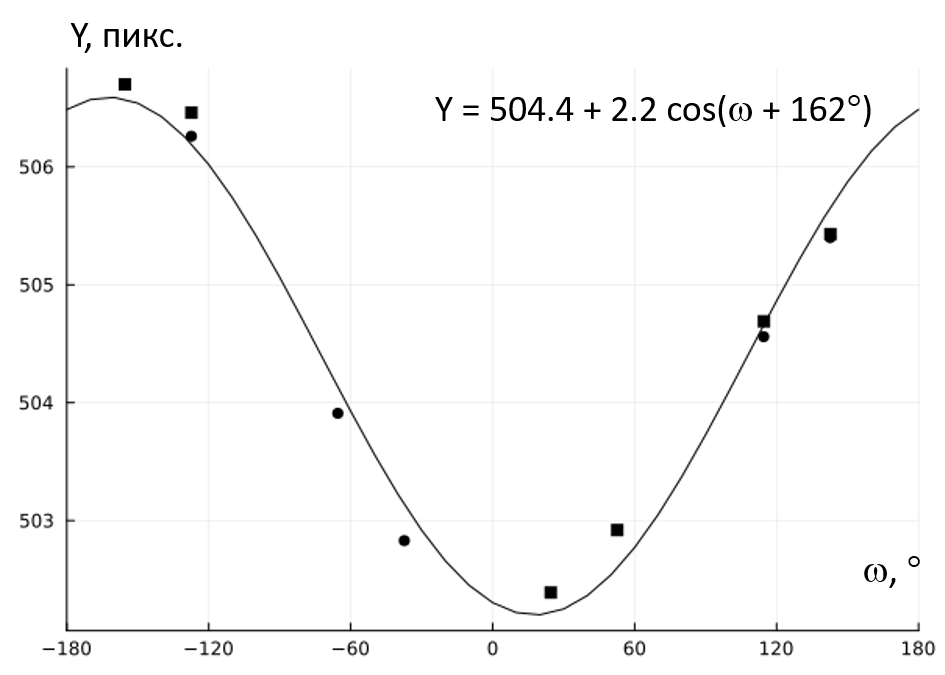
\includegraphics[width=0.8\textwidth]{eccentrGe.png}
    \caption{Зависимость координаты $Y$ от угла $\omega$ для монокристалла Ge. Для отрицательных (темные маркеры) и положительных (светлые маркеры) значениях $2\theta$ от значений $\omega$ были отняты значения $\theta + 90\degree$, тем самым позволив одновременно обработать все рефлексы. Аппроксимация функцией $Y = a_0 + a_1 \cos(\omega - \omega_1)$ выполнена с помощью МНК.}
    \label{fig:eccentrGe}
\end{figure}